\subsection{THE EULER INTEGRALS}

For brevity we shall say that a function \(f\) defined on an interval \(I \subset \mathbf{R}\) , and \(> 0\) on this interval, is logarithmically convex on \(I\) if \(\log f\) is convex on \(I\) . The definition of \(\Gamma(x)\) shows that this function is logarithmically convex on \(]0, +\infty[\) .

It is clear that the product of two logarithmically convex functions on I is also logarithmically convex on I. Further:

Lemma 1. Let \(f\) and \(g\) be two functions \(> 0\) and twice differentiable on an open interval I. If \(f\) and \(g\) are logarithmically convex functions on I, then \(f + g\) is logarithmically convex on I.

The relation \(\mathrm{D}^{2}\left(\log f(x)\right) \geqslant 0\) can be written \(f(x)f''(x) - \left(f'(x)\right)^{2} \geqslant 0\) . We are reduced to showing that the relations a \textgreater{} 0, \(a' > 0\) , \(ac - b^{2} \geqslant 0\) , \(a'c' - b'^{2} \geqslant 0\) imply \((a + a')(c + c') - (b + b')^{2} \geqslant 0\) ; now, when a \textgreater{} 0, the relation \(ac - b^{2} \geqslant 0\) is equivalent to the fact that the quadratic form \(ax^{2} + 2bxy + cy^{2}\) is \(\geqslant 0\) on \(R^{2}\) , and it is clear that if

\[
a x ^ {2} + 2 b x y + c y ^ {2} \geqslant 0 \quad \text { and } \quad a ^ {\prime} x ^ {2} + 2 b ^ {\prime} x y + c ^ {\prime} y ^ {2} \geqslant 0
\]

on \(\mathbf{R}^{2}\) then also \((a + a')x^{2} + 2(b + b')xy + (c + c')y^{2} \geqslant 0\) on \(\mathbf{R}^{2}\) .

Lemma 2. Let \(f\) be a finite real function, \(>0\) , defined and continuous on the product \(I \times J\) of two open intervals of \(\mathbf{R}\) , and such that, for every \(t \in J\) the function \(x \mapsto f(x,t)\) is logarithmically convex and twice differentiable on \(I\) . Under these hypotheses, if the integral \(g(x) = \int_{J} f(x,t) dt\) converges for every \(x \in I\) , then \(g\) is logarithmically convex on \(I\) .

First we show that for every compact interval \(K \subset J\) the function \(g_{K}(x) = \int_{K} f(x, t) dt\) is logarithmically convex. Indeed, if \(K = [a, b]\) , the sequence of functions

\[
g _ {n} (x) = \frac {b - a}{n} \sum_ {k = 0} ^ {n - 1} f \left(x, a + k \frac {b - a}{n}\right)
\]

converges simply to \(g_{K}(x)\) on I (II, p.~57, prop. 5) hence \(\log g_{n}\) converges simply to \(\log g_{K}\) ; by lemma 1 of VII, p.~310, \(\log g_{n}\) is convex on I, so (I, p.~27, prop. 4) it is the same for \(\log g_{K}\) .

On the other hand, g is the pointwise limit of the \(g_{K}\) along the directed set of compact subintervals of I (II, p.~64), so \(\log g\) is the pointwise limit of the \(\log g_{K}\) ; these last functions being convex on I, so is \(\log g\) (I, p.~27, prop. 4).

One can show easily that lemmas 1 and 2 remain valid even when one does not assume that the functions are twice differentiable (VII, p.~327, exerc. 5).

Lemma 3. Let \(\varphi\) be a continuous function and \(>0\) on an open interval \(J\) contained in \([0, +\infty[\) . If \(I\) is an open interval such that the integral \(g(x) = \int_{J} t^{x-1} \varphi(t) dt\) converges for all \(x \in I\) , then \(g\) is logarithmically convex on \(I\) .

Indeed, \(\log t^{x - 1} = (x - 1)\log t\) is a function of \(x\) which is convex and twice differentiable for all \(t > 0\) , so lemma 2 applies.

PROPOSITION 3. For all \(x > 0\)

\[
\Gamma (x) = \int_ {0} ^ {\infty} e ^ {- t} t ^ {x - 1} d t\tag{14}
\]

(second Euler integral).

Now the function \(g(x) = \int_0^\infty e^{-t} t^{x-1} dt\) is defined for all \(x > 0\) (V, p.~229); lemma 3 of VII, p.~311, then shows that it is logarithmically convex on \(]0, +\infty[\) . Moreover, on integrating by parts, one has

\[
g (x + 1) = \int_ {0} ^ {\infty} e ^ {- t} t ^ {x} d t = - e ^ {- t} t ^ {x} \Big | _ {0} ^ {\infty} + x \int_ {0} ^ {\infty} e ^ {- t} t ^ {x - 1} d t = x g (x).
\]

In other words, g is a solution of equation (1) of VII, p.~305; finally,

\[
g (1) = \int_ {0} ^ {\infty} e ^ {- t} d t = 1;
\]

the proposition therefore follows from prop. 1 of VII, p.~306.

By the change of variable \(e^{-t}=u\) one deduces from (14) (VII, p.~311) the formula

\[
\Gamma (x) = \int_ {0} ^ {1} \left(\log \frac {1}{t}\right) ^ {x - 1} d t.\tag{15}
\]

Similarly, from the change of variable \(u = t^{x}\) we obtain

\[
x \Gamma (x) = \int_ {0} ^ {\infty} e ^ {- t ^ {1 / x}} d t
\]

or again, taking account of (7) (VII, p.~3),

\[
\Gamma \left(1 + \frac {1}{x}\right) = \int_ {0} ^ {\infty} e ^ {- t ^ {x}} d t\tag{16}
\]

and in particular, for \(x = 2\)

\[
\Gamma \left(\frac {3}{2}\right) = \frac {1}{2} \Gamma \left(\frac {1}{2}\right) = \int_ {0} ^ {\infty} e ^ {- t ^ {2}} d t.\tag{17}
\]

PROPOSITION 4. For x \textgreater{} 0 and y \textgreater{} 0 the integral

\[
\mathbf {B} (x, y) = \int_ {0} ^ {1} t ^ {x - 1} (1 - y) ^ {y - 1} d t
\]

(first Euler integral) has the value

\[
\mathbf {B} (x, y) = \frac {\Gamma (x) \Gamma (y)}{\Gamma (x + y)}.\tag{18}
\]

Indeed this integral converges for \(x > 0\) and \(y > 0\) (V, p.~229). By lemma 3 of VII, p.~311, the function \(x \mapsto \mathbf{B}(x, y)\) is logarithmically convex for \(x > 0\) . Moreover,

\[
\mathbf {B} (x + 1, y) = \int_ {0} ^ {1} (1 - t) ^ {x + y - 1} \left(\frac {t}{1 - t}\right) ^ {x} d t
\]

whence, on integrating by parts,

\[
\begin{array}{l} \mathbf {B} (x + 1, y) = - \frac {(1 - t) ^ {x + y}}{x + y} \left(\frac {t}{1 - t}\right) ^ {x} \Bigg | _ {0} ^ {1} \\ \qquad + \frac {x}{x + y} \int_ {0} ^ {1} (1 - t) ^ {x + y} \left(\frac {t}{1 - t}\right) ^ {x - 1} \frac {d t}{(1 - t) ^ {2}} = \frac {x}{x + y} \mathbf {B} (x, y). \end{array}
\]

It follows that \(f(x) = \mathbf{B}(x, y) \Gamma(x + y)\) satisfies the identity (1) of VII, p.~305. Moreover, this function is logarithmically convex, being the product of two logarithmically convex functions. Finally, one has \(f(1) = \mathbf{B}(1, y) \Gamma(y + 1)\) , and \(\mathbf{B}(1, y) = \int_{0}^{1} (1 - t)^{y - 1} dt = 1/y\) , whence \(f(1) = \frac{1}{y} \Gamma(y + 1) = \Gamma(y)\) . The function \(f(x)/\Gamma(y)\) is thus equal to \(\Gamma(x)\) by prop. 1 of VII, p.~306, which proves (18).

By the change of variable \(t = \frac{u}{u + 1}\) the formula (18) becomes

\[
\int_ {0} ^ {\infty} \frac {t ^ {x - 1}}{(1 + t) ^ {x + y}} d t = \frac {\Gamma (x) \Gamma (y)}{\Gamma (x + y)}\tag{19}
\]

and by the change of variable \(t = \sin^{2} \varphi\)

\[
\int_ {0} ^ {\pi / 2} \sin^ {2 x - 1} \varphi \cos^ {2 y - 1} \varphi d \varphi = \frac {1}{2} \frac {\Gamma (x) \Gamma (y)}{\Gamma (x + y)}.\tag{20}
\]

If one puts \(x = y = \frac{1}{2}\) in this last formula it follows that

\[
\Gamma (\frac {1}{2}) = \sqrt {\pi}\tag{21}
\]

whence, by (17),

\[
\int_ {0} ^ {\infty} e ^ {- t ^ {2}} d t = \frac {1}{2} \sqrt {\pi}.\tag{22}
\]

From the relation (7) of VII, p.~307, one has the asymptotic expansion

\[
\begin{array}{l} \Gamma (x) = \frac {1}{x} \Gamma (x + 1) \\ = \frac {1}{x} + \Gamma^ {\prime} (1) + \frac {1}{2 !} \Gamma^ {\prime \prime} (1) x + \dots + \frac {1}{n !} \Gamma^ {(n)} (1) x ^ {n - 1} + O (x ^ {n}) \end{array}\tag{23}
\]

for \(\Gamma(x)\) , on a neighbourhood of 0.

Similarly, for all y fixed and \textgreater{} 0 one can write

\[
\begin{array}{l} \frac {1}{\Gamma (x + y)} = \frac {1}{\Gamma (y)} + D \left(\frac {1}{\Gamma (y)}\right) x \\ \qquad + \frac {1}{2 !} D ^ {2} \left(\frac {1}{\Gamma (y)}\right) x ^ {2} + \dots + \frac {1}{n !} D ^ {n} \left(\frac {1}{\Gamma (y)}\right) x ^ {n} + O _ {1} (x ^ {n + 1}) \end{array}
\]

and the formula (18) then gives, for y fixed, the asymptotic expansion

\[
\begin{array}{l} \mathbf {B} (x, y) = \frac {1}{x} + \left(\Gamma^ {\prime} (1) - \frac {\Gamma^ {\prime} (y)}{\Gamma (y)}\right) \\ \qquad + \left(\frac {\Gamma^ {\prime \prime} (1)}{2} - \Gamma^ {\prime} (1) \frac {\Gamma^ {\prime} (y)}{\Gamma (y)} + \frac {2 \Gamma^ {\prime 2} (y) - \Gamma (y) \Gamma^ {\prime \prime} (y)}{2 \Gamma^ {2} (y)}\right) x + O (x ^ {2}) \end{array}\tag{24}
\]

on a neighbourhood of \(x = 0\) .

Moreover, for x \textgreater{} 0 and y \textgreater{} 0 one has

\[
\begin{array}{l} \mathbf {B} (x, y) = \int_ {0} ^ {1} \left(t ^ {x - 1} + t ^ {x} \frac {(1 - t) ^ {y - 1} - 1}{t}\right) d t \\ = \frac {1}{x} + \int_ {0} ^ {1} t ^ {x} \frac {(1 - t) ^ {y - 1} - 1}{t} d t. \end{array}\tag{25}
\]

The function \(\varphi(t) = \frac{(1 - t)^{y - 1} - 1}{t}\) is continuous on the compact interval {[}0, 1{]}; since

\[
t ^ {x} = e ^ {x \log t} = 1 + x \log t + \frac {x ^ {2}}{2 !} (\log t) ^ {2} + \dots + \frac {x ^ {n}}{n !} (\log t) ^ {n} + r _ {n} (x, t)
\]

with \(|r_n(x,t)| \leqslant \frac{x^{n+1}}{(n+1)!} |\log t|^{n+1}\) (since \(\log t \leqslant 0\) and \(x > 0\) ), formula (25) gives the asymptotic expansion

\[
\begin{array}{l} \mathbf {B} (x, y) = \frac {1}{x} + \int_ {0} ^ {1} \varphi (t) d t + x \int_ {0} ^ {1} \varphi (t) \log t d t + \dots \\ \qquad + \frac {x ^ {n}}{n !} \int_ {0} ^ {1} \varphi (t) (\log t) ^ {n} d t + O _ {2} (x ^ {n + 1}) \end{array}
\]

for \(\mathbf{B}(x,y)\) on a neighbourhood of 0.

For \(n = 1\) the identification of this expansion with (24) gives in particular

\[
\Gamma^ {\prime} (1) - \frac {\Gamma^ {\prime} (y)}{\Gamma (y)} = \int_ {0} ^ {1} \frac {(1 - t) ^ {y - 1} - 1}{t} d t.
\]

Furthermore, the formula (10) gives \(\Gamma'(1) = \Gamma'(1)/\Gamma(1) = -\gamma\) , so (Gauss' integral)

\[
\frac {\Gamma^ {\prime} (x)}{\Gamma (x)} + \gamma = \int_ {0} ^ {1} \frac {1 - (1 - t) ^ {x - 1}}{t} d t.\tag{26}
\]

\section{THE GAMMA FUNCTION IN THE COMPLEX DOMAIN}

\subsection{EXTENDING THE GAMMA FUNCTION TO C}

Let us return to Weierstrass' formula which gives the expression

\[
\frac {1}{\Gamma (x)} = x e ^ {\gamma x} \prod_ {n = 1} ^ {\infty} \left(1 + \frac {x}{n}\right) e ^ {- x / n}\tag{1}
\]

for \(1 / \Gamma (x)\) for all real \(x\) , and consider the infinite product with general term \(\left(1 + \frac{z}{n}\right)e^{-z / n}\) for arbitrary complex \(z\) . One can write \(e^{-z / n} = 1 - \frac{z}{n} + h(z)\) , with \(|h(z)| \leqslant \frac{|z|^2}{2n^2} e^{|z / n|}\) (III, p.~106, formula (8)), whence

\[
\left(1 + \frac {z}{n}\right) e ^ {- z / n} = 1 + v _ {n} (z)
\]

with \(|v_{n}(z)| \leqslant \frac{|z|^{2}}{n^{2}}\left(1 + \frac{e^{|z|}}{2}(1 + |z|)\right)\) ; thus the infinite product under consideration is absolutely and uniformly convergent on every compact subset of C; further, its value is zero only at the points z = -n (Gen.~Top., IX, p.~214, corollary). In view of the formula (1) of VII, p.~315, for every complex z one puts

\[
\frac {1}{\Gamma (z)} = z e ^ {\gamma z} \prod_ {n = 1} ^ {\infty} \left(1 + \frac {z}{n}\right) e ^ {- z / n}.\tag{2}
\]

The function \(\Gamma(z)\) is thus defined for every point \(z \in \mathbf{C}\) apart from the points \(-n\) ( \(n \in \mathbf{N}\) ); it is continuous on this set, and \((z + n)\Gamma(z) \sim \frac{(-1)^n}{n!}\) on a neighbourhood of \(-n\) . Formula (2) shows that one has \(\Gamma(\overline{z}) = \overline{\Gamma(z)}\) for every \(z\) different from a negative integer.

The argument that allows one to pass from Gauss' formula (VII, p.~307, formula (8)) to Weierstrass' formula, on reversing the steps, applies also to complex \(z\) and shows that, for \(z \neq -n\) ( \(n \in \mathbf{N}\) ), one has

\[
\Gamma (z) = \lim _ {n \rightarrow \infty} \frac {n ^ {z} n !}{z (z + 1) \dots (z + n)}\tag{3}
\]

on agreeing to put \(n^z = e^{z\log n}\) . Since

\[
\frac {n ^ {z + 1} n !}{(z + 1) (z + 2) \dots (z + n + 1)} = z \frac {n}{n + 1 + z} \frac {n ^ {z} n !}{z (z + 1) \dots (z + n)}
\]

one again has, on passing to the limit, the fundamental functional equation

\[
\Gamma (z + 1) = z \Gamma (z)\tag{4}
\]

for every \(z \neq -n (n \in \mathbf{N})\) .

Let \(p\) be an arbitrary integer \(> 0\) , and \(\mathrm{K}_p\) the open disc \(|z| < p\) ; for every \(z \in \mathrm{K}_p\) , and every integer \(n > p\) , \(1 + \frac{z}{n}\) is not a negative real number, so \(\log \left(1 + \frac{z}{n}\right)\) is defined, and it follows from the above that the series with general term \(\log \left(1 + \frac{z}{n}\right) - \frac{z}{n} (n > p)\) is normally convergent on \(\mathrm{K}_p\) ; the same holds for the series obtained by differentiating the general term a finite number of times, since one has

\[
\left| \frac {1}{n} - \frac {1}{z + n} \right| \leqslant \frac {p}{n (n - p)} \quad \text { and } \quad \left| \frac {1}{(z + n) ^ {k}} \right| \leqslant \frac {1}{(n - p) ^ {k}} \quad (k > 1)
\]

for \(z \in \mathbf{K}_p\) and \(n > p\) . One then sees (cf.~II, p.~59, Remark 3) that \(\Gamma(z)\) is indefinitely differentiable at all the points \(z \in \mathbf{C}\) apart from the points \(-n\) , and at these points one has

\[
{\frac {\Gamma^ {\prime} (z)}{\Gamma (z)}} = - \gamma - {\frac {1}{z}} + \sum_ {n = 1} ^ {\infty} \left({\frac {1}{n}} - {\frac {1}{z + n}}\right)\tag{5}
\]

\[
\mathrm{D} ^ {k - 1} \left(\frac {\Gamma^ {\prime} (z)}{\Gamma (z)}\right) = \sum_ {n = 0} ^ {\infty} \frac {(- 1) ^ {k} (k - 1) !}{(z + n) ^ {k}} \quad \text { for } \quad k \geqslant 2,\tag{6}
\]

the right-hand sides of (5) and (6) being normally convergent on every compact subset of \(\mathbf{C}\) that does not contain any integer \(\leqslant 0\) . Further, one can write

\[
\log \Gamma (z) \equiv - \gamma z - \log z + \sum_ {n = 1} ^ {\infty} \left(\frac {z}{n} - \log \left(1 + \frac {z}{n}\right)\right) \pmod {2 \pi i}\tag{7}
\]

agreeing that when a logarithm in this formula is that of a real negative number it has one or the other limit values (differing by \(2\pi i\) ) of \(\log z\) at this point; the series on the right-hand side of (7) is then normally convergent on every compact subset of C not containing any integer \(\leqslant 0\) .

\subsection{THE COMPLEMENTS' RELATION AND THE LEGENDRE-GAUSS MULTIPLICATION FORMULA}

One derives immediately from formula (2) of VII, p.~315, that, for every \(z \in C\) ,

\[
\frac {1}{\Gamma (z) \Gamma (- z)} = - z ^ {2} \prod_ {n = 1} ^ {\infty} \left(1 - \frac {z ^ {2}}{n ^ {2}}\right).
\]

Now the Euler expansion of \(\sin z\) (VI, p.~287, th. 2) shows that

\[
z \prod_ {n = 1} ^ {\infty} \left(1 - \frac {z ^ {2}}{n ^ {2}}\right) = \frac {1}{\pi} \sin \pi z;
\]

taking account of the functional equation (4) of VII, p.~315, one then sees that:

PROPOSITION 1. For every complex \(z\) one has

\[
\frac {1}{\Gamma (z) \Gamma (1 - z)} = \frac {1}{\pi} \sin \pi z\tag{8}
\]

(the complements' relation).

COROLLARY --- For every real t one has

\[
| \Gamma (i t) | = \sqrt {\frac {\pi}{t \sinh \pi t}} \qquad (t \neq 0)\tag{9}
\]

\[
\left| \Gamma (\frac {1}{2} + i t) \right| = \sqrt {\frac {\pi}{\cosh \pi t}}.\tag{10}
\]

Indeed, one deduces from (8) that \(\Gamma(it)\Gamma(-it) = \frac{i\pi}{t\sin\pi it} = \frac{\pi}{t\sinh\pi t}\) , and one has \(\Gamma(-it) = \overline{\Gamma(it)}\) ; similarly, (8) gives

\[
\Gamma \left(\frac {1}{2} + i t\right) \Gamma \left(\frac {1}{2} - i t\right) = \frac {\pi}{\sin \left(\frac {\pi}{2} + \pi i t\right)} = \frac {\pi}{\cos \pi i t} = \frac {\pi}{\cosh \pi t},
\]

and one has

\[
\Gamma \bigl (\frac {1}{2} - i t \bigr) = \overline {{\Gamma \bigl (\frac {1}{2} + i t \bigr)}}.
\]

Now let \(p\) be any integer \(> 0\) and consider the product

\[
f (z) = \Gamma \left(\frac {z + 1}{p}\right) \Gamma \left(\frac {z + 2}{p}\right) \dots \Gamma \left(\frac {z + p}{p}\right).
\]

By (3) (VII, p.~315), for every \(z \neq -n\) ( \(n \in \mathbf{N}\) ), \(f(z)\) is the limit of the product

\[
\begin{array}{c} \frac {n ^ {(z + 1) / p} n !}{\left(\frac {z + 1}{p}\right) \left(\frac {z + 1}{p} + 1\right) \cdots \left(\frac {z + 1}{p} + n\right)}. \\ \frac {n ^ {(z + 2) / p} n !}{\left(\frac {z + 2}{p}\right) \left(\frac {z + 2}{p} + 1\right) \cdots \left(\frac {z + 2}{p} + n\right)} \dots \\ \dots \frac {n ^ {(z + p) / p} n !}{\left(\frac {z + p}{p}\right) \left(\frac {z + p}{p} + 1\right) \cdots \left(\frac {z + p}{p} + n\right)} \\ = \frac {n ^ {z + (p + 1) / 2} p ^ {(n + 1) p} (n !) ^ {p}}{(z + 1) (z + 2) \ldots (z + (n + 1) p)} \end{array}
\]

and in particular \(f(0)\) is the limit of the product

\[
\frac {n ^ {(p + 1) / 2} p ^ {(n + 1) p} (n !) ^ {p}}{((n + 1) p) !}
\]

from which it follows that \(f(z) / f(0)\) is the limit of

\[
\begin{array}{c} \frac {n ^ {z} ((n + 1) p) !}{(z + 1) (z + 2) \dots (z + (n + 1) p)} \\ = z   p ^ {- z} \left(\frac {n}{n + 1}\right) ^ {z}. \frac {((n + 1) p) ^ {z} ((n + 1) p) !}{z (z + 1) (z + 2) \dots (z + (n + 1) p)} \end{array}
\]

which, by (3) (VII, p.~315), gives

\[
f (z) = f (0) z p ^ {- z} \Gamma (z).\tag{11}
\]

But one can write

\[
f (0) = \prod_ {k = 1} ^ {p - 1} \Gamma \left(\frac {k}{p}\right) = \prod_ {k = 1} ^ {p - 1} \Gamma \left(1 - \frac {k}{p}\right) = \sqrt {\prod_ {k = 1} ^ {p - 1} \Gamma \left(\frac {k}{p}\right) \Gamma \left(1 - \frac {k}{p}\right)}
\]

since \(f(0) > 0\) ; the complements' relation then gives

\[
f (0) = \sqrt {\pi^ {p - 1} / \prod_ {k = 1} ^ {p - 1} \sin \frac {k \pi}{p}}
\]

and since the product on the right-hand side is equal to \(p/2^{p-1}\) (VI, p.~284, cor. 1) one sees finally that:

PROPOSITION 2. For every complex number z not an integer \(\leqslant 0\) and for every integer p \textgreater{} 0 one has

\[
\Gamma \left(\frac {z}{p}\right) \Gamma \left(\frac {z + 1}{p}\right) \dots \Gamma \left(\frac {z + p - 1}{p}\right) = (2 \pi) ^ {(p - 1) / 2} p ^ {\frac {1}{2} - z} \Gamma (z)\tag{12}
\]

(Legendre-Gauss multiplication formula).

PROPOSITION 3. For every real x \textgreater{} 0 one has

\[
\int_ {x} ^ {x + 1} \log \Gamma (t) d t = x (\log x - 1) + \frac {1}{2} \log 2 \pi\tag{13}
\]

(Raabe's integral).

First we establish formula (13) for \(x = 0\) . Since \(\log \Gamma(x) \sim \log \frac{1}{x}\) as \(x\) tends to 0, the integral \(\int_0^1 \log \Gamma(x) dx\) converges. Further, the function \(\log \Gamma(x)\) decreases on {[}0, 1{]} (VII, p.~310); for every \(\alpha > 0\) one thus has

\[
\frac {1}{n} \sum_ {k = 1} ^ {q} \log \Gamma \left(\frac {k}{n}\right) \leqslant \int_ {0} ^ {\alpha} \log \Gamma (x) d x,
\]

\(q\) being the largest integer such that \(q / n \leqslant \alpha\) . Since \(\int_{0}^{\alpha} \log \Gamma(x) dx\) tends to 0 with \(\alpha\) and also \(\frac{1}{n} \sum_{k=q+1}^{n} \log \Gamma\left(\frac{k}{n}\right)\) tends to \(\int_{\alpha}^{1} \log \Gamma(x) dx\) as \(n\) tends to \(+\infty\) (II, p.~57, prop. 5) one has

\[
\int_ {0} ^ {1} \log \Gamma (x) d x = \lim _ {n \rightarrow \infty} \frac {1}{n} \sum_ {k = 1} ^ {n} \log \Gamma \left(\frac {k}{n}\right).
\]

But, by (12), the right-hand side of this formula is the limit of

\[
\frac {n - 1}{2 n} \log 2 \pi - \frac {1}{2} \frac {\log n}{n},
\]

whence

\[
\int_ {0} ^ {1} \log \Gamma (x) d x = \frac {1}{2} \log 2 \pi .\tag{14}
\]

Next we remark that from the identity

\[
\log \Gamma (x + 1) = \log \Gamma (x) + \log x
\]

one deduces, on integrating, that for x \textgreater{} 0

\[
\int_ {0} ^ {x} \log \Gamma (t + 1) d t = \int_ {0} ^ {x} \log \Gamma (t) d t + \int_ {0} ^ {x} \log t d t.
\]

But the integral on the left-hand side is also equal to \(\int_{1}^{x + 1}\log \Gamma (t)dt\) . Thus, by (14),

\[
\int_ {x} ^ {x + 1} \log \Gamma (t) d t = \int_ {0} ^ {x} \log t d t + \frac {1}{2} \log 2 \pi = x (\log x - 1) + \frac {1}{2} \log 2 \pi .
\]

\subsection{STIRLING'S EXPANSION}

Let \(x\) and \(y\) be two complex numbers not lying on the real negative half-axis; by formula (3) of VII, p.~315, with the conventions of VII, p.~316, concerning the logarithms, \(\log \Gamma(x) - \log \Gamma(y)\) is congruent modulo \(2\pi i\) to the limit of the expression

\[
(x - y) \log n + \sum_ {k = 0} ^ {n} \Big (\log (y + k) - \log (x + k) \Big).\tag{15}
\]

Let us put \(f(t) = \log(y + t) - \log(x + t)\) ; we apply the Euler-Maclaurin summation formula (VI, p.~288) to the function f:

\[
\begin{array}{l} f (0) + f (1) + \dots + f (n) = \int_ {0} ^ {n + 1} f (t) d t - \frac {1}{2} \big (f (n + 1) - f (0) \big) \\ \qquad + \sum_ {k = 1} ^ {p} \frac {b _ {2 k}}{(2 k) !} \big (f ^ {(2 k - 1)} (n + 1) - f ^ {(2 k - 1)} (0) \big) + T _ {p} (n) \end{array}
\]

with

\[
\left| \mathrm{T} _ {p} (n) \right| \leqslant \frac {4 e ^ {2 \pi}}{(2 \pi) ^ {2 p + 1}} \int_ {0} ^ {n + 1} \left| f ^ {(2 p + 1)} (u) \right| d u.\tag{16}
\]

Since

\[
f ^ {(m)} (t) = (- 1) ^ {m - 1} (m - 1)! \left(\frac {1}{(y + t) ^ {m}} - \frac {1}{(x + t) ^ {m}}\right),
\]

\(f^{(2k - 1)}(n + 1)\) tends to 0 as \(n\) tends to \(+\infty\) , for all \(k \geqslant 1\) ; it is the same for

\[
f (n + 1) = \log \left(1 + \frac {y}{n + 1}\right) - \log \left(1 + \frac {x}{n + 1}\right).
\]

Moreover, one has

\[
\int_ {0} ^ {n + 1} \log (x + t) d t = (x + n + 1) (\log (x + n + 1) - 1) - x (\log x - 1);
\]

as n tends to \(+\infty\) , one has the asymptotic expansion

\[
(x + n) \bigl (\log (x + n) - 1 \bigr) = n \log n - n + x \log n + O \left(\frac {1}{n}\right).
\]

Substituting in the expression (15) one sees finally that, as n tends to \(+\infty\) , \(\mathrm{T}_{p}(n)\) has a limit \(\mathrm{R}_{p}(x, y)\) and that one can write

\[
\log \Gamma (x) - g (x) \equiv \log \Gamma (y) - g (y) + \mathrm{R} _ {p} (x, y)\tag{mod.  \( 2\pi i \)}
\]

on putting

\[
g (x) = x \log x - x - \frac {1}{2} \log x + \sum_ {k = 1} ^ {p} \frac {b _ {2 k}}{2 k (2 k - 1)} \frac {1}{x ^ {2 k - 1}}.\tag{17}
\]

We shall now evaluate a bound for \(\mathrm{R}_{p}(x,y)\) with the help of (16), assuming that x and y are both in the subset \(H_{A}\) of C defined by the relation `` \(\mathcal{R}(z)\geqslant A\) or \(|\mathcal{I}(z)|\geqslant A\) '', where A is an arbitrary number \textgreater0 (fig.~2). To this end we remark that if \(x=s+it\) with s\textgreater A one has \(|x+u|\geqslant A+u\) for every u\textgreater0, and consequently

\[
\int_ {0} ^ {n + 1} \frac {d u}{| x + u | ^ {2 p + 1}} \leqslant \int_ {0} ^ {\infty} \frac {d u}{(\mathrm{A} + u) ^ {2 p + 1}} = \frac {1}{2 p \mathrm{A} ^ {2 p}}.
\]

Similarly, if \(|t| \geqslant A\) one has \(|x + u| = |s + u + it| \geqslant \sqrt{A^2 + (s + u)^2}\) for all real \(u\) , whence

\[
\int_ {0} ^ {n + 1} \frac {d u}{| x + u | ^ {2 p + 1}} \leqslant \int_ {- \infty} ^ {+ \infty} \frac {d u}{(\mathrm{A} ^ {2} + u ^ {2}) ^ {p + 1 / 2}} = \frac {2}{\mathrm{A} ^ {2 p}} \int_ {0} ^ {\infty} \frac {d v}{(1 + v ^ {2}) ^ {p + 1 / 2}}.
\]

Thus one sees that, when x and y are in \(H_{A}\) , one has

\[
\left| \mathrm{R} _ {p} (x, y) \right| \leqslant \frac {\mathrm{C} _ {p}}{\mathrm{A} ^ {2 p}}
\]

\pandocbounded{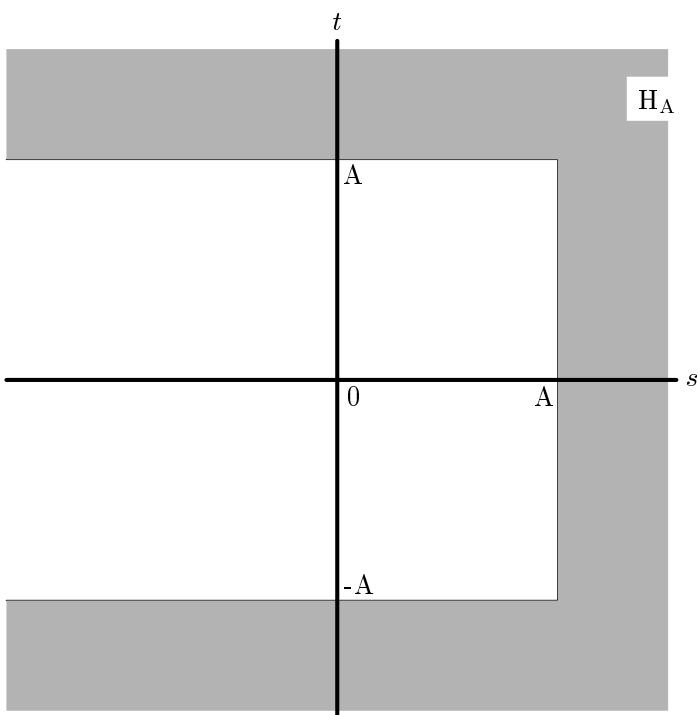
\includegraphics[keepaspectratio]{images/part002_194eed20.jpg}}\\
Fig. 2

where \(C_{p}\) depends only on p.~Now let F be the filter having the sets \(H_{A}\) as basis; the Cauchy criterion shows that, along the filter F, the function \(\log \Gamma(z) - g(z)\) has a finite limit \(\delta\) (modulo \(2\pi i\) ) and that, if one puts \(\omega(z) = \max(\mathcal{R}(z), |\mathcal{I}(z)|)\) , one has

\[
\log \Gamma (z) - g (z) - \delta \equiv O \left(\frac {1}{(\omega (z)) ^ {2 p}}\right) \pmod {2 \pi i}.\tag{18}
\]

For \(x\) real and \(> 0\) one has \(\Gamma(x) > 0\) , and \(g(x)\) is real, so one can assume that \(\delta\) is real and one has

\[
\log \Gamma (x) = g (x) + \delta + O \left(\frac {1}{x ^ {2 p}}\right).
\]

Now we shall deduce the value of the constant \(\delta\) ; by prop. 2 of VII, p.~318, applied for p = 2, one has, for real x tending to \(+\infty\)

\[
\begin{array}{c} \frac {x - 1}{2} \log \frac {x}{2} - \frac {x}{2} + \frac {x}{2} \log \frac {x + 1}{2} - \frac {x + 1}{2} + 2 \delta \\ = x \log x - x - \frac {1}{2} \log x + (\frac {1}{2} - x) \log 2 + \frac {1}{2} \log 2 \pi + \delta + o (1) \end{array}
\]

from which one deduces easily that \(\delta = \frac{1}{2}\log 2\pi\) . Finally one has the following result:

PROPOSITION 4. Along the filter \(\mathfrak{F}\) one has (for every integer \(p \geqslant 1\) ) the asymptotic expansion

\[
\begin{array}{l} \log \Gamma (z) \equiv z \log z - z - \frac {1}{2} \log z + \frac {1}{2} \log 2 \pi \\ \quad + \sum_ {k = 1} ^ {p} \frac {b _ {2 k}}{2 k (2 k - 1)} \frac {1}{z ^ {2 k - 1}} + O \left(\frac {1}{(\omega (z)) ^ {2 p}}\right) \pmod {2 \pi i} \end{array}\tag{19}
\]

(Stirling's expansion).

COROLLARY. Along the filter F one has

\[
\Gamma (z) \sim \sqrt {2 \pi} \exp (z \log z - z - \frac {1}{2} \log z).\tag{20}
\]

In particular, for \(x\) real tending to \(+\infty\) the formula (20) can be written

\[
\Gamma (x) \sim \sqrt {2 \pi} x ^ {x - 1 / 2} e ^ {- x},\tag{21}
\]

whence, as the integer n tends to \(+\infty\) ,

\[
n! \sim \sqrt {2 \pi} n ^ {n + 1 / 2} e ^ {- n}
\]

(cf.~V, p.~244).

One can deduce numerous formulae from this. For example, for every complex number \(\alpha\) and every integer n one has, as n tends to \(+\infty\) ,

\[
\frac {\Gamma (n + \alpha)}{\Gamma (n)} \sim n ^ {\alpha} \quad (= e ^ {\alpha \log n}).\tag{22}
\]

Similarly, for every complex number a not an integer \(\leqslant 0\) one has

\[
a (a + 1) (a + 2) \dots (a + n) = \frac {\Gamma (n + a + 1)}{\Gamma (a)} \sim \frac {\sqrt {2 \pi}}{\Gamma (a)} n ^ {n + a + 1 / 2} e ^ {- n}\tag{23}
\]

and for every complex number a not an integer \(\geqslant 0\)

\[
\binom {a} {n} = \frac {(- 1) ^ {n}}{\Gamma (- a)}   \frac {\Gamma (n - a)}{\Gamma (n + 1)} \sim \frac {(- 1) ^ {n}}{\Gamma (- a)}   n ^ {- a - 1}.\tag{24}
\]

Finally, for every real constant \(k > 1\) one has

\[
\binom {k n} {n} = \frac {\Gamma (k n + 1)}{\Gamma (n + 1)   \Gamma ((k - 1) n + 1)} \sim \sqrt {\frac {k}{2 \pi (k - 1) n}} \left(\frac {k ^ {k}}{(k - 1) ^ {k - 1}}\right) ^ {n}.\tag{25}
\]

The same argument leads to the following analogous proposition:

PROPOSITION 5. Along the filter \(\mathfrak{F}\) one has (for every integer \(p \geqslant 1\) ), the asymptotic expansion

\[
\frac {\Gamma^ {\prime} (z)}{\Gamma (z)} = \log z - \frac {1}{2 z} - \sum_ {k = 1} ^ {p} \frac {b _ {2 k}}{2 k} \frac {1}{z ^ {2 k}} + O \left(\frac {1}{(\omega (z)) ^ {2 p + 1}}\right).\tag{26}
\]

Instead of prop. 2 of VII, p.~318, one uses the formula

\[
\int_ {x} ^ {x + 1} \frac {\Gamma^ {\prime} (t)}{\Gamma (t)} d t = \log \Gamma (x + 1) - \log \Gamma (x) = \log x
\]

in order to determine the constant.

\setcounter{exercisegroup}{0}
\refstepcounter{exercisegroup}
\section*{Exercises on \S\arabic{exercisegroup}}
\phantomsection
\addcontentsline{toc}{section}{Exercises on \protect\S\arabic{exercisegroup}}

J 1) Let \(g\) be a regulated function, and \(>0\) on \(]0, +\infty[\) .

\begin{enumerate}
\def\labelenumi{\alph{enumi})}
\tightlist
\item
  Let \(u, v\) be two increasing functions on \(]0, +\infty[\) such that \(u(x + 1) - u(x) = v(x + 1) - v(x) = g(x)\) for all \(x > 0\) . Show that if \(w = u - v\) one has
\end{enumerate}

\[
\sup _ {0 <   x \leqslant y \leqslant 1} | w (y) - w (x) | \leqslant \inf _ {x > 0} g (x).
\]

(Remark that, for \(a \leqslant x \leqslant y \leqslant a + 1\) one has \(u(y) - u(x) \leqslant g(a)\) .) In particular, if \(\inf_{x > 0} g(x) = 0\) there exists at most one increasing solution of the equation \(u(x + 1) - u(x) = g(x)\) taking a given value at a given point.

\begin{enumerate}
\def\labelenumi{\alph{enumi})}
\setcounter{enumi}{1}
\tightlist
\item
  Assume that g is decreasing on {]}0, +∞{[}. Show that the series
\end{enumerate}

\[
\varphi (x) = - g (x) + \sum_ {n = 1} ^ {\infty} (g (n) - g (x + n))
\]

is absolutely and uniformly convergent on every compact interval contained in {]}0, +∞{[}; if \(\lambda = \lim_{x \to +\infty} g(x)\) then the function \(u(x) = \varphi(x) + \lambda x\) is an increasing solution of the equation \(u(x+1) - u(x) = g(x)\) . Show that for every increasing solution v of this equation one has \(v(y) - v(x) \geqslant \varphi(y) - \varphi(x)\) for 0 \textless{} x \textless{} y. What is the upper (resp. lower) envelope of the set of increasing solutions of the equation \(u(x+1) - u(x) = g(x)\) taking a given value at a given point? Show that this set reduces to a single element if and only if \(\lambda = 0\) . c) Show that if \(g(x)\) is increasing and \textgreater0 on {[}0, +∞{]} there are infinitely many increasing solutions of the equation \(u(x+1) - u(x) = g(x)\) which take a given value at a given point. d) Let \(\psi(x)\) be the function defined on {]}0, +∞{[} by the conditions: \(\psi(x)=0\) for \(0\leqslant x<1\) , \(\psi(x)=1\) for \(1\leqslant x<2\) , \(\psi(x)=n\) for \(n-1+\frac{1}{n-1}\leqslant x<n+\frac{1}{n}\) ( \(n\geqslant2\) ); let \(g(x)=\psi(x+1)-\psi(x)\) . Show that \(\psi\) is the unique increasing solution of the equation

\[
u (x + 1) - u (x) = g (x)
\]

such that \(u(1)=1\) .

J2) Let g be a continuous increasing function on {]}0, +∞{[}.

\begin{enumerate}
\def\labelenumi{\alph{enumi})}
\item
  Show that if \(\liminf_{x\to +\infty}g(x) / x = 0\) there exists at most one convex solution of the equation \(u(x + 1) - u(x) = g(x)\) taking a given value at a given point (remark that for all \(h > 0\) the function \(v(x) = u(x + h) - u(x)\) is an increasing function satisfying the equation \(v(x + 1) - v(x) = g(x + h) - g(x)\) , and apply exerc. 1 a)).
\item
  Show that if g is concave on \(]0, +\infty[\) there exists a convex solution of the equation \(u(x+1) - u(x) = g(x)\) ; there exists a unique convex solution of this equation taking a given value at a given point if and only if \(\lim_{x \to +\infty} g(x)/x = 0\) (cf.~exerc. 1 b)).
\item
  Suppose from here on that \(g\) is increasing and concave on \(]0, +\infty[\) , and that \(\lim_{x \to +\infty} g(x) / x = 0\) . For every pair of numbers \(h > 0\) , \(k > 0\) and every finite real function \(f\) defined on \(]0, +\infty[\) one puts
\end{enumerate}

\[
\varDelta \Big (f (x); h, k \Big) = \frac {f (x + h) - f (x)}{h} - \frac {f (x) - f (x - k)}{k}
\]

for x \textgreater{} k. Show that if u is a convex solution of the equation \(u(x + 1) - u(x) = g(x)\) , one has \(\lim_{x \to +\infty} \Delta(u(x); h, k) = 0\) for all h \textgreater{} 0 and k \textgreater{} 0 (use the expression for \(u_{r}^{\prime}\) from exerc. 1 b) of VII, p.~325).

\(d\) ) With the notation of \(c\) ) show that there exists a constant \(\alpha\) such that one has \(u(x) = v(x) + \alpha\) , with

\[
v (x) = \int_ {1} ^ {x} g (t) d t - \frac {1}{2} g (x) + R (x)
\]

where we have put

\[
\mathrm{R} (x) = \sum_ {n = 0} ^ {\infty} h (x + n), \quad h (x) = \int_ {x} ^ {x + 1} g (t) d t - \frac {1}{2} (g (x + 1) + g (x));
\]

further, one has

\[
0 \leqslant \mathrm{R} (x) \leqslant \frac {1}{2} (g (x + \frac {1}{2}) - g (x)).
\]

(Remark that \(v(x + 1) - v(x) = g(x)\) and that \(\lim_{x\to +\infty}\Delta (v(x);h,k) = 0\) irrespective of \(h > 0\) and \(k > 0\) .)

\begin{enumerate}
\def\labelenumi{\arabic{enumi})}
\setcounter{enumi}{2}
\tightlist
\item
  \begin{enumerate}
  \def\labelenumii{\alph{enumii})}
  \tightlist
  \item
    Let g be a function defined and admitting a continuous \(k^{th}\) derivative on {]}0, +∞{[}, such that \(g^{(k)}\) is decreasing on this interval and that \(\lim_{x\to+\infty}g^{(k)}(x)=0\) . Show that there exists one and only one solution u of the equation \(u(x+1)-u(x)=g(x)\) which admits an increasing \(k^{th}\) derivative on {]}0, +∞{[} and takes a given value at a given point (use exerc. 1 b)).
  \end{enumerate}
\end{enumerate}

\begin{enumerate}
\def\labelenumi{\alph{enumi})}
\setcounter{enumi}{1}
\tightlist
\item
  Let \(\alpha\) be an arbitrary real number. Let \(S_{\alpha}\) be the function defined on \(]0, +\infty[\) satisfying the relation
\end{enumerate}

\[
\mathrm{S} _ {\alpha} (x + 1) - \mathrm{S} _ {\alpha} (x) = x ^ {\alpha}
\]

such that \(S_{\alpha}(1) = 0\) , and, further, that the derivative of \(S_{\alpha}\) of order equal to the integer part of \((\alpha + 1)^{+}\) is increasing (it is a unique function by \(a\) )). Show that

\[
\mathrm{S} _ {\alpha} ^ {\prime} (x) - \mathrm{S} _ {\alpha} ^ {\prime} (1) = \alpha \mathrm{S} _ {\alpha - 1} (x),
\]

and

\[
\mathrm{S} _ {\alpha} \left(\frac {x}{p}\right) + \mathrm{S} _ {\alpha} \left(\frac {x + 1}{p}\right) + \dots + \mathrm{S} _ {\alpha} \left(\frac {x + p - 1}{p}\right) = \frac {1}{p ^ {\alpha}} \mathrm{S} _ {\alpha} (x) + \mathrm{C} _ {\alpha}
\]

for every integer \(p \geqslant 1\) , where \(C_{\alpha}\) is a constant, which, when \(\alpha \neq -1\) , is equal to

\[
\left(\frac {1}{p ^ {\alpha}} - p\right) \frac {S _ {\alpha + 1} ^ {\prime} (1)}{\alpha + 1}
\]

(cf.~VII, p.318, prop. 2 and VI, p.~291, exerc. 3).

\begin{enumerate}
\def\labelenumi{\arabic{enumi})}
\setcounter{enumi}{3}
\tightlist
\item
  Show that the function \(f(x) = \frac{1}{\sqrt{2}}\frac{\Gamma(x / 2)}{\Gamma\left(\frac{x + 1}{2}\right)}\) is the unique convex solution of the
\end{enumerate}

equation \(u(x + 1) = 1 / x \, u(x)\) (remark that this equation implies \(u(x + 2) = \frac{x}{x + 1} \, u(x)\) and apply exerc. 1 a)).

\begin{enumerate}
\def\labelenumi{\arabic{enumi})}
\setcounter{enumi}{4}
\item
  Generalize lemmas 1 and 2 of VII, p.~310 and 311, to arbitrary logarithmically convex functions (cf.~I, p.~45, exerc. 2). Show that every logarithmically convex function is convex.
\item
  Let \(\psi(x) = \Gamma'(x)/\Gamma(x)\) ; for every integer \(q > 1\) and every integer \(k\) such that \(1 \leqslant k \leqslant q - 1\) establish the formulae
\end{enumerate}

\[
\sum_ {p = 1} ^ {q} \psi \left(\frac {p}{q}\right) \exp \left(\frac {2 p k \pi i}{q}\right) = - q \sum_ {n = 1} ^ {\infty} \frac {1}{n} \exp \left(\frac {2 n k \pi i}{q}\right) = q \log \left(1 - \exp \frac {2 k \pi i}{q}\right).
\]

(Use formula (9) of VII, p.~307.)

\setcounter{exercisegroup}{1}
\refstepcounter{exercisegroup}
\section*{Exercises on \S\arabic{exercisegroup}}
\phantomsection
\addcontentsline{toc}{section}{Exercises on \protect\S\arabic{exercisegroup}}

\(\mathfrak{J}1)\) a) Let \(g\) be a continuous real function for \(x \geqslant 0\) . Show that if \(g\) satisfies the two identities

\[
\sum_ {k = 0} ^ {p - 1} g \left(\frac {x + k}{p}\right) = g (x)
\]

\[
\sum_ {h = 0} ^ {q - 1} g \left(\frac {x + h}{q}\right) = g (x)
\]

it also satisfies the identity

\[
\sum_ {j = 0} ^ {p q - 1} g \left(\frac {x + j}{p q}\right) = g (x).
\]

\begin{enumerate}
\def\labelenumi{\alph{enumi})}
\setcounter{enumi}{1}
\tightlist
\item
  Deduce from this that if a function \(g\) has a continuous derivative for \(x \geqslant 0\) and satisfies the identity
\end{enumerate}

\[
\sum_ {k = 0} ^ {p - 1} g \left(\frac {x + k}{p}\right) = g (x)
\]

then it is of the form \(a(x-\frac{1}{2})\) , where a is a constant (remark that g satisfies the analogous identity where p is replaced by \(p^{n}\) ; let n tend to \(+\infty\) and deduce that \(g'(x)=\int_{0}^{1}g'(t)dt\) ). c) Conclude from b) that the \(\Gamma\) function is the only function having a continuous derivative for x\textgreater0, which satisfies equation (1) of VII, p.~305, and the multiplication formula (12) of VII, p.~318, for a value of p.

\begin{enumerate}
\def\labelenumi{\arabic{enumi})}
\setcounter{enumi}{1}
\tightlist
\item
  For every integer \(k > 1\) put \(S_k = \sum_{n=1}^{\infty} n^{-k}\) . Show that, for \(-1 < x \leqslant 1\) one has
\end{enumerate}

\[
\log \Gamma (1 + x) = - \gamma x + \sum_ {k = 2} ^ {\infty} (- 1) ^ {k} \frac {\mathrm{S} _ {k}}{k} x ^ {k}
\]

the series on the right being uniformly convergent on every compact subset of \(]-1,1]\) , and absolutely convergent for \(|x|<1\) .

\begin{enumerate}
\def\labelenumi{\arabic{enumi})}
\setcounter{enumi}{2}
\tightlist
\item
  Let s be a fixed real number; show that when t tends to \(+\infty\) or to \(-\infty\) one has
\end{enumerate}

\[
| \Gamma (s + i t) | \sim \sqrt {2 \pi} | t | ^ {s - 1 / 2} e ^ {- (\pi / 2) | t |}
\]

and

\[
\frac {\Gamma^ {\prime} (s + i t)}{\Gamma (s + i t)} \sim \log | t |.
\]

\begin{enumerate}
\def\labelenumi{\arabic{enumi})}
\setcounter{enumi}{3}
\tightlist
\item
  Let t be a fixed real number \(\neq 0\) ; show that as s tends to \(+\infty\)
\end{enumerate}

\[
| \Gamma (- s + i t) | \sim \sqrt {\frac {\pi}{2}} \left(s ^ {s + 1 / 2} e ^ {- s} \sqrt {\sinh^ {2} \pi t + \sin^ {2} \pi s}\right) ^ {- 1}
\]

(use the complements' relation).

\begin{enumerate}
\def\labelenumi{\arabic{enumi})}
\setcounter{enumi}{4}
\tightlist
\item
  Let \(x_{n}\) be the root of the equation \(\Gamma'(x) = 0\) in the interval \(] - n, -n + 1[\) . Show that
\end{enumerate}

\[
x _ {n} = - n + \frac {1}{\log n} + O \left(\frac {1}{(\log n) ^ {2}}\right)
\]

(use the complements' relation and formula (5) of VII, p.~316). Deduce that

\[
\Gamma (x _ {n}) \sim \frac {(- 1) ^ {n}}{\sqrt {2 \pi}} n ^ {- n - 1 / 2} e ^ {n + 1} \log n.
\]

\begin{enumerate}
\def\labelenumi{\arabic{enumi})}
\setcounter{enumi}{5}
\tightlist
\item
  Let \(V_{n}\) be the Vandermonde determinant \(\mathrm{V}(1,2,\dots,n)\) (Alg., III, p.~532). Show that
\end{enumerate}

\[
\log V _ {n} = \frac {n ^ {2}}{2} \log n - \frac {3 n ^ {2}}{4} + \left(\frac {1}{2} \log 2 \pi - \frac {1}{4}\right) n - \frac {1}{12} \log n + k + O \left(\frac {1}{n}\right)
\]

where k is a constant.

\section*{Historical Note}
\phantomsection
\addcontentsline{toc}{section}{Historical Note}

(N.B. Roman numerals refer to the bibliography to be found at the end of this note.)

The idea of ``interpolating'' a sequence \((u_{n})\) by the values of an integral depending on a real parameter \(\lambda\) and equal to \(u_{n}\) for \(\lambda = n\) , goes back to Wallis (III, p.~55). It was this idea that principally guided Euler when, in 1730 ((I), v. XIV, p.~1-24) he set himself to interpolate the sequence of factorials. He began by remarking that \(n!\) is equal to the infinite product \(\prod_{k=1}^{\infty}\left(\frac{k+1}{k}\right)^{n}\frac{k}{k+n}\) , which product is defined for every value of n (an integer or not), and that in particular, for the value \(n = \frac{1}{2}\) it takes the value \(\frac{1}{2}\sqrt{\pi}\) by Wallis' formula. The analogy between this result and Wallis' led him then to revisit the integral

\[
\int_ {0} ^ {1} x ^ {e} (1 - x) ^ {n} d x
\]

(n integral, e arbitrary) already considered by the latter. Euler obtained the value \(\frac{n!}{(e+1)(e+2)\ldots(e+n+1)}\) for it, using the Binomial expansion; a change of variables then showed him that \(n!\) is the limit, as z tends to 0, of the integral \(\int_{0}^{1}\left(\frac{1-x^{z}}{z}\right)^{n}dx\) , whence the ``second Euler integral''

\[
n! = \int_ {0} ^ {1} \left(\log \frac {1}{x}\right) ^ {n} d x;
\]

by the same method, and using Wallis' formula, he obtained the formula \(\int_0^1\sqrt{\log 1 / x} dx = \frac{1}{2}\sqrt{\pi}\) . In his later works Euler often returned to these integrals; he thus discovered the complements' relation ((I), t. XV, p.~82 and t. XVII, p.~342), the formula \(\mathbf{B}(p,q) = \Gamma (p)\Gamma (q) / \Gamma (p + q)\) ((I), t. XVII, p.~355), and the particular case of the Legendre-Gauss formula corresponding to \(x = 1\) ((I), t. XIX, p.~483); all this of course without worrying about questions of convergence.

Gauss pursued the study of the \(\Gamma\) function in connection with his research on the hypergeometric function, of which the \(\Gamma\) function is a limit case (II); it was in the course of this research that he obtained the general multiplication formula (already noted by Legendre a little earlier for p = 2). The later work on \(\Gamma\) was mainly concerned with extending this function to the complex domain. Only recently has it been appreciated that the property of logarithmic convexity characterises \(\Gamma(x)\) (in the real domain), up to a constant factor, among the solutions of the functional equation \(f(x + 1) = x f(x)\) (III); and Artin showed (IV) how one can link all the classical results on \(\Gamma(x)\) simply to this property. We have followed his exposition quite closely.

\section*{Bibliography}
\phantomsection
\addcontentsline{toc}{section}{Bibliography}

\begin{enumerate}
\def\labelenumi{(\Roman{enumi})}
\item
  L. EULER, Opera omnia, Leipzig-Berlin (Teubner): t. XIV (1924), t. XV (1927), t. XVII (1915) and t. XIX (1932).
\item
  C.F. GAUSS, Werke, t. III, Göttingen, 1866.
\item
  H. BOHR und J. MOLLERUP, Laerebog i matematisk Analyse, t. III, Kopenhagen, 1922, p.~149-164.
\item
  E. ARTIN, Einführung in die Theorie der Gammafunktion, Leipzig (Teubner), 1931.
\end{enumerate}

\backmatter
\chapter*{Index of Notation}
\phantomsection
\addcontentsline{toc}{chapter}{Index of Notation}

\begin{Shaded}
\begin{Highlighting}[]
\FunctionTok{Df(x0)}\KeywordTok{:}\AttributeTok{ }\DecValTok{5}
\FunctionTok{f\textquotesingle{}(x0)}\KeywordTok{:}\AttributeTok{ }\DecValTok{5}
\FunctionTok{f\textquotesingle{}d(x0)}\KeywordTok{:}\AttributeTok{ }\DecValTok{6}
\FunctionTok{f\textquotesingle{}g(x0)}\KeywordTok{:}\AttributeTok{ }\DecValTok{6}
\FunctionTok{Df}\KeywordTok{:}\AttributeTok{ }\DecValTok{7}
\FunctionTok{df/dx}\KeywordTok{:}\AttributeTok{ }\DecValTok{7}
\FunctionTok{f\textquotesingle{}d}\KeywordTok{:}\AttributeTok{ }\DecValTok{7}
\FunctionTok{f\textquotesingle{}g}\KeywordTok{:}\AttributeTok{ }\DecValTok{7}
\FunctionTok{D\^{}n f}\KeywordTok{:}\AttributeTok{ }\DecValTok{23}
\FunctionTok{f(n)}\KeywordTok{:}\AttributeTok{ }\DecValTok{23}
\FunctionTok{∫x0 f}\KeywordTok{:}\AttributeTok{ }\DecValTok{61}
\FunctionTok{∫x0 f(t) dt}\KeywordTok{:}\AttributeTok{ }\DecValTok{61}
\FunctionTok{∫x0\^{}x f}\KeywordTok{:}\AttributeTok{ }\DecValTok{61}
\FunctionTok{∫x0\^{}x f(t) dt}\KeywordTok{:}\AttributeTok{ }\DecValTok{61}
\FunctionTok{h(t)|x|\_\{x0\}}\KeywordTok{:}\AttributeTok{ }\DecValTok{62}
\FunctionTok{∫a(n) f}\KeywordTok{:}\AttributeTok{ }\DecValTok{66}
\FunctionTok{∫I f(t) dt}\KeywordTok{:}\AttributeTok{ }\DecValTok{69}
\FunctionTok{e}\KeywordTok{:}\AttributeTok{ }\DecValTok{97}
\FunctionTok{exp x}\KeywordTok{:}\AttributeTok{ }\DecValTok{97}
\FunctionTok{log x (x real \textgreater{} 0)}\KeywordTok{:}\AttributeTok{ }\DecValTok{97}
\FunctionTok{π}\KeywordTok{:}\AttributeTok{ }\DecValTok{99}
\FunctionTok{Arc cos x}\KeywordTok{:}\AttributeTok{ }\DecValTok{100}
\FunctionTok{Arc sin x}\KeywordTok{:}\AttributeTok{ }\DecValTok{100}
\FunctionTok{Arc tan x}\KeywordTok{:}\AttributeTok{ }\DecValTok{100}
\FunctionTok{cos x}\KeywordTok{:}\AttributeTok{ }\DecValTok{100}
\FunctionTok{cot x}\KeywordTok{:}\AttributeTok{ }\DecValTok{100}
\FunctionTok{csc x}\KeywordTok{:}\AttributeTok{ }\DecValTok{100}
\FunctionTok{sec x}\KeywordTok{:}\AttributeTok{ }\DecValTok{100}
\FunctionTok{sin x}\KeywordTok{:}\AttributeTok{ }\DecValTok{100}
\FunctionTok{tan x}\KeywordTok{:}\AttributeTok{ }\DecValTok{100}
\FunctionTok{e\^{}z}\KeywordTok{:}\AttributeTok{ }\DecValTok{103}
\FunctionTok{exp z}\KeywordTok{:}\AttributeTok{ }\DecValTok{103}
\FunctionTok{cos z}\KeywordTok{:}\AttributeTok{ }\DecValTok{107}
\end{Highlighting}
\end{Shaded}

cot z: 107 log z: 105 sin z: 107 tan z: 107 cosh x: 108 sinh x: 108 tanh x: 108 Arg cosh x: 109 Arg sinh x: 109 Arg tanh: 110 \(\binom{m}{n}\) : 114 \(e^{A}\) : 198 exp A: 198 \(\mathcal{H}(\mathfrak{F}, V)\) : 221 \(R_{\infty}\) : 221 \(\mathcal{H}_{\infty}(\mathfrak{F}, V)\) : 222 \(f_{1} \preccurlyeq f_{2}\) : 223 \(f_{2} \succcurlyeq f_{1}\) : 223 \(f \preccurlyeq g\) : 223 \(g \succcurlyeq f\) : 223 \(f + g\) : 223 fg: 223 fλ: 223 \textbar\textbar f\textbar\textbar: 223 f ≃ g: 224 \(f_{1} \prec f_{2}\) : 225 \(f_{2} \succcurlyeq f_{1}\) : 225 \(f \prec g\) : 225 \(g \succcurlyeq f\) : 225 f \textasciitilde{} g: 226 \(O(f), O_{k}(f), o(f), o_{k}(f)\) : 230 \(l_{0}(x), l_{n}(x)\) : 240 \(\mathfrak{K}(y) (\mathfrak{K} \text{ a Hardy field})\) : 261 \(e_{0}(x), e_{n}(x)\) : 265 \(\sum_{k=0}^{\infty} \alpha_{k} D^{k}\) : 285 \(B_{n}(X)\) : 288 \(b_{n}\) : 288 \(U_{x}^{\xi}(f(\xi))\) : 290 \(\Gamma(n), \Gamma(x)\) : 317 B (x, y): 324 \(\Gamma(z)\) : 327

\chapter*{Index}
\phantomsection
\addcontentsline{toc}{chapter}{Index}

\par\noindent\textbf{\texorpdfstring{wlog\textbackslash indfile=\textbackslash read1}{wlog=}}\par

Adjoining a root of a polynomial, of a primitive, of an exponential of a primitive, to a differential field, 121

Adjoint (equation) of a differential linear equation, 186

Appell polynomials, 272

Approximate solution to within \(\varepsilon\) of a differential equation, 166

Asymptotic expansion

- more precise than another, 222

- of a function relative to a comparison scale, 222

- of a function to precision \(g_{\alpha}\) , 222

- precision of, 222

Asymptotic expansions, 220

- with variable coefficients, 226

\par\noindent\textbf{Bernouilli numbers, 276}\par

Bernouilli polynomials, 275

Binomial formula, 108

Binomial series, 109

Carleman's inequality, 117

Carlson inequality, 116

Cauchy's criterion for integrals, 65

Change of variables formula, 60

Character

- local, 211

Coefficients

- binomial, 21

Comparison scales, 220

Complements' relation, 316

Composition operator, 270

- indicatrix, 278

- order of, 272

- regular, 279

Cosecant, 95

Cosine

- hyperbolic, 102

Cosine of a complex number, 102

Cotangent, 95

Criteria

- convergence

-- of the second kind, 244

- integrals

-- logarithmic, 229

Criterion

- Cauchy's criterion for integrals, 65

-- Cauchy-Maclaurin, 237

- Ermakoff's, 86

\par\noindent\textbf{d'Alembert}\par

-- criterion for convergence, 245

Definition sequence for an (H) function, 252

Derivative

- first, 3

- infinite, 10

- logarithmic, 94

- \(n^{th}\) , 20

- second, 20

- symmetric, 39

Derivative of a function, 3

- left, 4

- right, 4

Determinant of \(n\) integrals of a system of \(n\) linear differential equations, 184

Differential equation

- adjoint, 187

- integral, 163

- linear, 177

- linear homogeneous, 178

- linear of order \(n\) , 192

- Lipschitz, 171

- locally Lipschitz, 171

- of first order, 164

- of order \(n\) , 164

-- real variable, 163

- scalar, 164

- solution, 163

\par\noindent\textbf{336}\par

\par\noindent\textbf{INDEX}\par

\par\noindent\textbf{Field}\par

- differential, 121 Formula - change of variables, 60 - Euler-Maclaurin summation, 282 - Gauss', 307 - integration by parts, 60 - integration by parts of order n, 60 - Legendre-Gauss multiplication, 318 - Leibniz', 20 - Stirling's, 243 - Taylor's, 21 - Wallis', 123 - Weierstrass', 308 Formulae - Euler's, 99 Function - n times differentiable -- at a point, 20 -- on an interval, 20 - (H), 252 - concave, 26 - convex, 26 - derived, 4 - differentiable -- at a point, 3 -- indefinitely, 20 -- on an interval, 4 - domination of one function by another, 212 - elementary, 122

Generalized Taylor expansion of a function, 278

Generalized Taylor expansion of a polynomial, 274

Generating series of the Appell polynomials attached to a composition operator, 275

Hadamard's inequality, 118

Hardy-Littlewood inequality, 89

Hardy-Littlewood tauberian theorem, 45

Hermite polynomials, 282

Hlawka's inequality, 90

Hyperbolic functions, 102

Hölder's inequality, 115

\par\noindent\textbf{Identity}\par

- Redheffer, 88

Indefinitely differentiable function, 20

Indicatrix of a composition operator, 278 Inequality

- Carleman's, 117

- Carlson, 116

-- Cauchy-Buniakowski-Schwarz, 115

- Cauchy-Schwarz, 88

- Hadamard's, 118

- Hardy, 117

- Hardy-Littlewood, 89

- Hlawka's, 90

- Hölder, 115

- Opial, 90

- Weyl, 90

Integral

- absolutely convergent, 67

- convergent, 63

- Euler, 310

- Gauss', 314

- normally convergent, 71, 73

- of a piecewise regulated function, 63

- of a regulated function over a

noncompact interval, 63

- of differential equation, 163

- Raabe's, 318

- uniformly convergent, 71

Integration by parts formula, 60

Integration by parts formula of order \(n\) , 60

Iterated exponentials, 253

Iterated logarithm, 229

\par\noindent\textbf{Kummer's congruences, 295}\par

\par\noindent\textbf{Leibniz' formula, 20}\par

Line

- locally above a graph, 31

- locally below a graph, 31

- locally on a graph, 31

Liouville's theorem, 122

Lipschitz condition, 168

Lipschitz differential equation, 171

Lipschitz function, 171

local character, 211

Logarithm

- iterated, 229

- Naperian, 92

- natural, 92

Maximum

- of complex number, 100

- principal value, 100

Logarithmic derivative, 94

Logarithmically bounded function, 214

Logarithmically convex function, 310

- relative, 11

-- strict, 11

\par\noindent\textbf{Mean}\par

- arithmetic, 93

-- weighted, 93

- geometric, 93

-- weighted, 93

Mean value of a function, 58

Mean value theorem, 14

Method of variation of parameters, 182

Minimum

- relative, 11

-- strict, 11

Naperian logarithm, 92

Natural logarithm, 92

Newton's polygon, 259

Normally convergent integral, 71

\par\noindent\textbf{Operator}\par

- composition, 270

- translation, 270

Opial inequality, 90

Order of one function with respect to another, 218

Peano's theorem, 167

Piecewise regulated function, 63

Polygon

- Newton, 259

Polynomials

- Appell, 272

- Bernouilli, 275

- Hermite, 282

Preponderant

- one function over another, 214

Prime number

- irregular, 295

- regular, 295

Primitive

- of a function on an interval of \(\mathbf{R}\) , 51

- of order \(n\) , 62

- second, 62

- strict, 51

Principal part

- of a function relative to a comparison scale, 221

- of a function relative to a comparison scale and a domain of coefficients, 227

Principle of comparison of integrals, 66

\par\noindent\textbf{INDEX}\par

Raabe's integral, 318

Raabe's test, 244

Redheffer identity, 88

Reduced to precision \(g_{\alpha}\)

- asymptotic expansion of a function, 222

Regular composition operator, 279

Regulated function, 54

\par\noindent\textbf{Remainder}\par

- in asymptotic expansion, 222

-- in the Euler-Maclaurin formula, 283

- in the Taylor formula, 22

Resolvent of a linear differential equation, 180

Rolle's theorem, 12

Roots

- characteristic, of a linear differential equation with constant coefficients, 190

Scales of comparison, 220

Secant, 95

Second mean value theorem, 82

Similar functions, 214

Sine

- hyperbolic, 102

Sine of a complex number, 102

Solution to within \(\varepsilon\) of a differential equation, 166

Stirling's formula, 243

Strict primitive, 51

Strict solution of a differential equation, 164

Strictly

- above a graph, 23

- below a graph, 23

Strictly concave function, 26

Strictly convex function, 25

Support line to graph of a convex function, 29

Systems

System of differential equations, 164 - fundamental systems of integrals of a linear system of scalar differential equations, 183

\par\noindent\textbf{Tangent}\par

- half

-- left, 11

-- right, 11

- hyperbolic, 102

- to a graph, 11

Taylor's expansion, 22

Taylor's formula, 21

- of order \(n\) , 22

\par\noindent\textbf{Test}\par

- d'Alembert's, 245

- Raabe's, 244

\par\noindent\textbf{Theorem}\par

- Cauchy's existence theorem, 171

-- Clausen-von Staudt, 294

-- Hardy-Littlewood tauberian, 45

- Liouville, 122

- Mean value, 14

- Peano, 167

- Rolle, 12

Theorems

- du Bois-Reymond, 265

Translation operator, 270

\par\noindent\textbf{Uniformly convergent integral, 71}\par

\par\noindent\textbf{Value}\par

- mean value of a function, 58

Variation of parameters

-method of, 182

Wallis' formula, 123

Weierstrass' formula, 308

Weyl inequality, 90

Wronskian of \(n\) integrals of a linear differential equation of order \(n\) , 193
